\chapter[SUAVIZAÇÃO DE MALHAS NÃO ESTRUTURADAS]{SUAVIZAÇÃO DE MALHAS NÃO ESTRUTURADAS}

Embora ferramentas de geração de malhas automáticas sejam amplamente usadas, essas ferramentas podem não garantir a qualidade das malhas. Não apenas no processo de tesselação, mas também no refinamento da malha, é possível que alguns elementos severamente distorcidos ou fora de forma sejam criados. Mesmo quando uma malha uniforme é desejada, a ferramenta de tesselação pode gerar elementos que são muito pequenos ou muito grandes comparados com os elementos desejados. \cite{Zhou}

Existem vários tipos de esquemas de suavização de malhas, tais como suavização Laplaciana e suavização baseada em otimização. Tipicamente cada método possui um compromisso entre qualidade e custo computacional. Por exemplo, a suavização Laplaciana requer um custo computacional muito baixo, mas frequentemente resulta em uma malha de baixa qualidade nos elementos ou mesmo com elementos inválidos. Por outro lado, enquanto suavizações baseados na otimização são mais prováveis em evitar elementos inválidos e obtém uma maior qualidade na malha, o custo computacional é muito maior que a suavização Laplaciana. \cite{Zhou}

\section{Suavização Centroidal Voronoi Tessellation}

O método \textit{centroidal Voronoi tesselation} é uma tesselação cujos pontos gerados são os centróides das regiões de Voronoi correspondentes. \cite{Du1999}

Dado um conjunto aberto $\Omega \subset \mathbb{R}^N$, o conjunto ${V_i}_{i=1}^k$ é chamado de uma tesselação de $\Omega$ se $V_i \cap V_j = \emptyset$ para $i \neq j$ e $\cup_{i=1}^k \hat{V_i} = \hat{\Omega}$.

Dado um conjunto de pontos ${z_i}_{i=1}^k$ pertencentes a $\hat{\Omega}$, a região de Voronoi $\hat{V_i}$ que corresponde aos pontos $z_i$ é definida por:

\begin{equation}
    \hat{V_i} = {x \in \Omega |  |x-z_i| < |x-z_j| \text{para} j=1,...,j, j \neq i }
\end{equation}

Os pontos ${z_i}_{i=1}^k$ são chamados de sementes. Enquanto que o conjunto ${\hat{V_i}}_{i=1}^k$ é chamado de diagrama de Voronoi de $\Omega$ e cada $\hat{V_i}$ se refere a região de Voronoi correspondente a $z_i$.

Pode-se entender um diagrama de Voronoi como um conjunto de células em que as fronteiras dessas células estão de tal forma que os pontos contidos nas células são os mais próximos de um ponto específico. Ou seja, um diagrama de Voronoi é uma maneira de particionar um plano em regiões conhecidas como células baseado na distância de um conjunto específico de pontos conhecidos como sementes. Cada célula possui uma semente e os pontos nessa célula estão mais próximos dessa semente do que qualquer outra semente. Além disso pode-se considerar as regiões de Voronoi como poliedros.

Dado uma região $V \subset \mathbb{R}^N$ e uma função densidade $\rho$, definida em $V$, o centróide de massa $z^*$ de $V$ é definido como:

\begin{equation}
    z^* = \frac{\int_V y \rho(y) dy}{\int_V \rho(y) dy}
\end{equation}

Dado $k$ pontos $z_i$, $i=1,...,k$ podemos definir as suas regiões de Voronoi associadas $\hat{V_i},i=1,...,k$. Por outro lado, dados as regiões $\hat{V_i},i=1,...,k$ podemos definir seus centros de massa $z_i^k,i=1,...,k$. Nesse caso, interessa a situação em que:

\begin{equation}
    z_i = z_i^*, i=1,...,k
\end{equation}

Ou seja, os pontos $z_i$ que servem como as sementes (ou geradores) das regiões de Voronoi $\hat{V_i}$ são também os centros de massa dessas regiões. Chama-se tal tesselação como "centroidal Voronoi tessellation". A diferença entre uma tesselação de Voronoi e uma tesselação de Voronoi centrada pode ser visualizada na figura \ref{fig:voronoi_tessellation}.

\begin{figure}
    \centering
    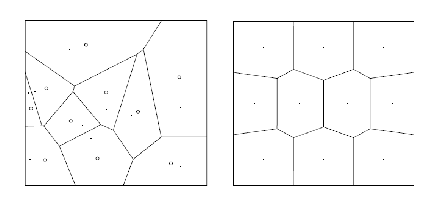
\includegraphics{fig/voronoi_tessellation.eps}
    \caption[Tesselação de Voronoi]{Tesselação de Voronoi}
    \label{fig:voronoi_tessellation}
\end{figure}

% \subsubsection{Fixed Point Uniform}

% O primeiro método de suavização de malha é chamado de Fixed Point Uniform e consiste em mover as sementes das células para o valor da média ponderada dos centroides das células vizinhas. Com essas novas sementes se refaz a tesselação de Voronoi e ligando-se os centroides das novas células, tem-se as triangulações de Delaunay.

\section{Suavização de Laplace}

A suavização de Laplace é o método mais comum e direto para suavisar uma malha. Ele apenas move cada nó para o centróide do polígono formado pelos nós adjacentes. Ele é um algoritmo de suavização local porque, em cada passo, o movimento do nó é calculado usando-se a localização dos seus nós adjacentes apenasa. Normalmente realiza-se a iteração apenas algumas vezes porque a qualidade da malha não é melhorada com novas iterações; de fato a qualidade pode, muitas vezes, piorar. \cite{Zhou}

Na suavização de Laplace nós podemos considerar a malha como um sistema de molas como mostrado na figura \ref{fig:laplacian_smoothing}. Cada aresta conectando ao nó central com os seus nós vizinhos podem ser vistos como um sistema linear de molas com um tamanho inicial de zero. Seja $\vec{v_i}$ o vetor do nó central com o i-ésimo nó vizinho:

\begin{equation*}
    \vec{v_i} = (x_i - x, y_i - y)
\end{equation*}

A soma das forças de mola agindo no nó central é:

\begin{equation*}
    \vec{F} = K \sum_{i=1}^k \vec{v_i}
\end{equation*}

Em que $K$ é a constante de mola, e $k$ é o número de nós vizinhos. Quando o nó central é localizado exatamente no centro geométrico do polígono, as forças de mola estão balanceadas e o sistema de mola está em equilíbrio.

Enquanto a suavização de Laplace é uma maneira iterativa de se achar este estado de forças balanceadas, nós podemos também resolver esse problema por minimização de energia do sistema de molas. Considerando que todas as molas tem um comprimento inicial de zero, nós podemos computar a energia potencial do sistema como:

\begin{equation*}
    E = \sum_{i=1}^k \frac{1}{2} K (||\vec{v_i}||)^2
\end{equation*}

Este é um problema de otimização, em que a função de custo é esta função quadrática, como mostrado na figura \ref{fig:energia-mola}. Minimizando-se esta função de custo nós podemos obter o mesmo resultado de se usar a suavização de Laplace.

A suavização de Laplace pode, portanto, ser vista como um tipo de otimização nodal local. A função de custo é a soma dos mínimos quadrados dos comprimentos das arestas compartilhadas pelo mesmo nó:

\begin{equation*}
    f(x,y) = \sum_{i=1}^k ((x-x_i)^2 + (y-y_i)^2)
\end{equation*}

Devido ao custo da função de suavização de Laplace ser o de uma função quadrática, ela se torna muito simples de achar a posição do nó que irá minimizar essa função. Podemos obter a posição $(x,y)$ que minimiza a função de custo simplesmente encontrando-se o centro geométrico dos nós vizinhos:

\begin{equation*}
    \frac{\partial f}{\partial x} = \frac{\partial f}{\partial y} = 0
\end{equation*}

\begin{equation*}
    x = \frac{1}{k} \sum_{i=1}^k x_i, y = \frac{1}{k} \sum_{i=1}^k y_i
\end{equation*}

Essa função de curso, no entaanto, não reflete necessariamente a qualidade da malha, e essa é a razão pela qual a suavização de Laplace frequentemente falha em melhorar a qualidade da malha, e em alguns casos, até mesmo gera elementos inválidos.

Abaixo está listado as vantagens e desvantagens da suavização de Laplace:

Vantagens:
\begin{itemize}
    \item Computacionalmente eficiente
    \item Fácil de ser implementada
\end{itemize}

Desvantagens:
\begin{itemize}
    \item Nem sempre move o nó para a posição ótima de modo a se obter o elemento de melhor qualidade
    \item Pode gerar elementos invertidos
    \item Tende a perder a uniformidade de tamanho caso a iteração rode mais que algumas vezes
    \item Tende a gerar elementos de menor qualidade caso a iteração rode mais que algumas vezes
\end{itemize}

\section{Suavização baseada em otimização}

Métodos baseados em suavização por otimização usam algumas medidas de qualidade da malha de modo a definir as funções de custo. Os nós da malha são movidos de modo a minimizar ou a maximizar essas funções.

Algumas funções de custo usadas nesse tipo de suavização são:

\begin{itemize}
    \item Mínimo/Máximo ângulo:\\
    O mínimo/máximo ângulo é um índice direto para se medir a qualidade da malha. Um elemento com ângulos próximos a 0º ou 180º irá criar dificuldades no processo de análise de elementos finitos. Na suavização baseada em otimização, portanto, ou o menor angulo é maximizado ou o maior angulo é minimizado de modo a se eliminar elementos severaamente distorcidos.
    \item Razão de proporção:\\
    A razão de proporção é a razão entre o raio do círculo circunscrito com o círculo inscrito do elemento de malha. Um triângulo equilateral tem uma razão de proporção de 2.0. Quando um elemento se torna muito distorcido, a razão de proporção aumenta.
    \item Métricas de distorção:\\
    As métricas de distorção estão relacionadas com a área e com o comprimento das fronteiras dos elementos. A qualidade do formato de um elemento pode ser verificado quantitativamente usando-se este tipo de métricas. Um triângulo equilateral tem o melhor valor possível, e um elemento muito distorcido tem um valor próximo a zero. Essas métricas podem também ser usadas em elementos quadrilaterais.
\end{itemize}

Uma das vantagens de suavizações baseadas em otimização é a que elas garantem uma melhora na qualidade da malha. Otimizando a qualidade das medidas, elementos severamente distorcidos são efetivamente elimidados. O custo computacional, no entanto, é muito maior do que a suavização de laplace. Para um elemento triangulos 2D, por exemplo, a suavização baseada em otimização pode ser cinco vezes mais caro computacionalmente que a suavização de Laplace esperta \cite{Freitag1997OnCL}, e 30 a 40 vezes mair caro computacionalmente que a suavização de Laplace.

\section{Suavização baseada na otimização de ângulos}

Segundo \cite{Zhou}, o método de suavização de malhas 2D baseado em ângulos compara cada nó da malha com os pares de ângulos adjacentes incidentes no nó e ajusta-se esses ângulos de modo que eles se tornam iguais no caso de uma malha triangular. No artigo é mostrado que essa técnica de suavização gera uma malha de maior qualidade em relação ao método da suavização Laplaciana e com um menor custo computacional.

\subsection{Algoritmo}
Esta seção descreve o algoritmo de suavização baseado em ângulos para uma malha triangular. A ideia central desse método é fazer com que cada par de ângulos adjacentes sejam iguais ou em uma certa razão, isso é eficaz para eliminar ângulos próximos a 0º ou 180º. Este método é fácil de ser implementado, e a qualidade da malha resultante é significativamente melhor que aplicando-se a suavização de Laplace, enquanto que o custo computacional é muito menor que as suavizações baseadas em otimização.

Nesse algoritmo, pode-se fazer uma analogia com um sistema de molas. A diferença entre este método e o método Laplaciano é que as molas usadas aqui são molas de torção. A energia potencial de tal sistema de molas de torção é:

\begin{equation*}
    E = \sum_{i=1}^{2k} \frac{1}{2} K \Theta_i^2
\end{equation*}

onde $k$ é o número de vértices do polígono, $K$ é a constante de mola e $\Theta$ é o ângulo na fronteira do polígono. Cada par de ângulos compartilha um vértice do polígono, portanto, existem $2k$ ângulos no total para serem considerados.

\begin{figure}[h]
    \centering
    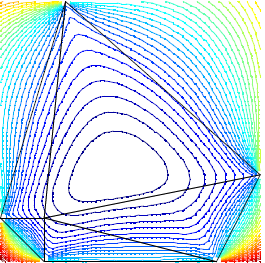
\includegraphics{fig/contorno-mola-torcao.png}
    \caption{Energia do sistema de molas de torção}
    \label{fig:contorno-mola-torcao}
\end{figure}

A plotagem do contorno dessa energia é mostrada na figura \ref{fig:contorno-mola-torcao}. É usado o mesmo polígono que a suavização de Laplace conforme a figura \ref{fig:energia-mola}. Comparando-se essas duas plotagens, nós encontramos que a posição de energia mínima é diferente nos dois casos. A suavização baseada em ângulos fornece uma melhor localização em relação ao método de Laplace.

É implementado um método iterativo que irá minimizar a energia potencial do sistema de molas de torção. O algoritmo de suavização baseado em ângulos é resumido nos seguintes cinco passos:

\begin{enumerate}
    \item Como mostrado na figura \ref{fig:angle-based}, para cada nó $N_i$, existem $k$ pares de ângulos ao redor dele, onde $k$ é o número de nós vizinhos. Os dois ângulos adjacentes são calculados como:
    
    \begin{equation*}
        \alpha_1 = \arccos{\qty(\frac{\vec{v_j} \cdot \vec{v_{j+1}}}{\norm{\vec{v_j}} \norm{\vec{v_{j+1}}} })}
    \end{equation*}
    \begin{equation*}
        \alpha_2 = \arccos{\qty(\frac{\vec{v_j} \cdot \vec{v_{j-1}}}{\norm{\vec{v_j}} \norm{\vec{v_{j-1}}} })}
    \end{equation*}

    Onde $\vec{v_{v-i}}$, $\vec{v_j}$ e $\vec{v_{j+1}}$ são vetores que compartilham o vértice $N_j$; $\norm{\vec{v}}$ é a norma $L_2$ do vetor; e $\alpha_1$, $\alpha_2$ são os ângulos determinados pelos três vetores.

    \begin{figure}[]
        \centering
        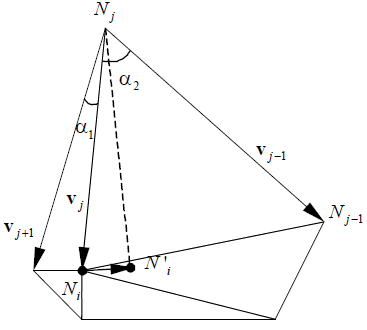
\includegraphics{fig/angle-based.png}
        \caption{Método de suavização baseado em ângulos}
        \label{fig:angle-based}
    \end{figure}

    \item Calcular a diferença entre dois ângulos adjacentes, e decidir qual o ângulo que o vetor $\vec{v_j}$ será rotacionado:
    
    \begin{equation*}
        \beta_j = (\alpha_2 - \alpha_1) / 2
    \end{equation*}

    Onde $\beta_j$ é o ângulo pelo qual o vetor $\vec{v_j}$ irá rotacionar.

    \item Rotacional o vetor $\vec{v_j}$ no ângulo $\beta_j$ ao redor de $N_j$, de modo que as novas coordenadas do nó $N_i$ serão:
    
    \begin{equation*}
    \begin{split}
        x' = x_0 + (x-x_0) \cos{\beta_j} - (y-y_0) \sin{\beta_j}\\
        y' = y_0 + (x-x_0) \sin{\beta_j} + (y-y_0) \cos{\beta_j}
    \end{split}
    \end{equation*}

    Onde $(x_0, y_0)$ é a localização do nó $N_j$, $(x,y)$ é a localização antiga do nó $N_i$ e $(x', y')$ é a nova localização do nó $N_i$.

    \item Iterando-se todos os nós vizinhos, existem $k$ conjuntos de novas localizações para o mesmo nó $N_i$. É computado agora a localização final do nó $N_i$ pegando-se a média de $(x', y')$ computada de todos os nós vizinhos.
    
    \begin{equation*}
    \begin{split}
        x_{new} = \frac{1}{k} \sum_{i=1}^k x'_i\\
        y_{new} = \frac{1}{k} \sum_{i=1}^k y'_i
    \end{split}
    \end{equation*}
\end{enumerate}

\section{Suavização Optimal Delaunay Tesselation}

\cite{Chen2011}